\documentclass[../main.tex]{subfiles}

\begin{document}

\section{Leírási módok}

\begin{fulltheorem}
  Mi az alapvető különbség az átviteli függvény és állapotváltozós leírási mód
  között? Mutassa be a lineáris idő invariáns rendszerek esetén az állapottér
  egyenletek rendszermátrixának sajátértékei és a rendszer átviteli
  függvényének pólusai közötti összefüggést.
\end{fulltheorem}

\begin{figure}[H]
  \centering
  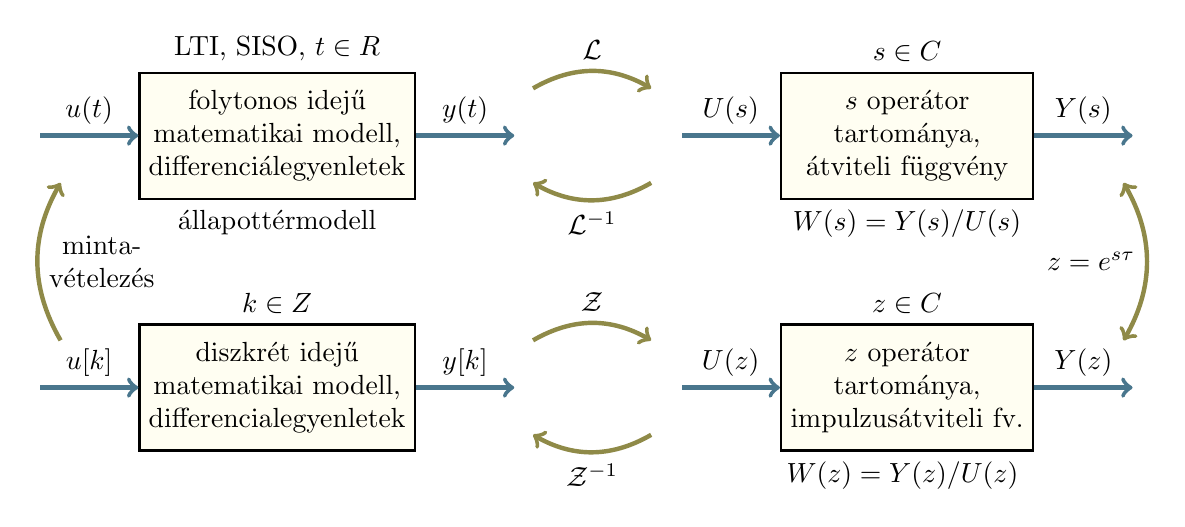
\begin{tikzpicture}[
      thick,
      box/.style={
          rectangle, draw=black, fill=yellow!5,
          minimum height=1.6cm, minimum width=3.2cm,
          align=center,
        },
      arr/.style={ultra thick, cyan!50!black},
      tr/.style={ultra thick, yellow!50!black},
    ]
    \node[box] (t) at (-4,+1.6) {
      % SISO, LTI, $t \in \mathbb R$ \\
      folytonos idejű \\ matematikai modell, \\
      differenciálegyenletek
    };
    \node[box] (k) at (-4,-1.6) {
      diszkrét idejű \\ matematikai modell, \\
      differencialegyenletek
    };

    \node[box] (s) at (+4,+1.6) {
      $s$ operátor \\ tartománya, \\
      átviteli függvény
    };
    \node[box] (z) at (+4,-1.6) {
      $z$ operátor \\ tartománya, \\
      impulzusátviteli fv.
    };

    % noindent
    \foreach \n/\l/\r/\a/\b in {
      t/{$u(t)$}/{$y(t)$}/{LTI, SISO, $t \in \mathbb R$}/{állapottérmodell},
      k/{$u[k]$}/{$y[k]$}/{$k \in \mathbb Z$}/{},
      s/{$U(s)$}/{$Y(s)$}/{$s \in \mathbb C$}/{$W(s) = Y(s) / U(s)$},
      z/{$U(z)$}/{$Y(z)$}/{$z \in \mathbb C$}/{$W(z) = Y(z) / U(z)$}
    }{
      \draw[arr, to-] (\n.west) -- ++(-1.25,0)
        node[midway, above, black] {\l};
      \draw[arr, -to] (\n.east) -- ++(+1.25,0)
        node[midway, above, black] {\r};
      \node[above] at (\n.north) {\a};
      \node[below, align=center] at (\n.south) {\b};
    }
    % indent

    \draw[tr, -to] (-.75,2.2) to[bend left]
    node[midway, above, black] {$\mathcal L$} ++(1.5,0);
    \draw[tr, to-] (-.75,1) to[bend right]
    node[midway, below, black] {$\mathcal L^{-1}$} ++(1.5,0);

    \draw[tr, -to] (-.75,-1) to[bend left]
    node[midway, above, black] {$\mathcal Z$} ++(1.5,0);
    \draw[tr, to-] (-.75,-2.2) to[bend right]
    node[midway, below, black] {$\mathcal Z^{-1}$} ++(1.5,0);

    \draw[tr, -to] (-6.75,-1) to[bend left]
    node[midway, right, black, align=center] {minta-\\vételezés} ++(0,2);
    \draw[tr, to-to] (6.75,-1) to[bend right]
    node[midway, left, black] {$z = e^{s \tau}$} ++(0,2);
  \end{tikzpicture}
  \caption{A leírási módok közötti kapcsolat}
  \label{fig:analogies-connection}
\end{figure}

\end{document}
